\documentclass[11pt]{article}

%%%%%%%%%%%%%%Include Packages%%%%%%%%%%%%%%%%%%%%%%%%%%
\usepackage{xcolor}
\usepackage{mathtools}
\usepackage[a4paper, total={6in, 8in}, margin=1.25in]{geometry}
\usepackage{amsmath}
\usepackage{amssymb}
\usepackage{paralist}
\usepackage{rsfso}
\usepackage{amsthm}
\usepackage{wasysym}
\usepackage[inline]{enumitem}   
\usepackage{hyperref}
\usepackage{tocloft}
\usepackage{titlesec}
\usepackage{colortbl}
%%%%%%%%%%%%%%%%%%%%%%%%%%%%%%%%%%%%%%%%%%%%%%%%%%%%%%%%



\begin{document}
\Large \noindent \textbf{Physics 5A Discussion (Week 0)}\\
\normalsize
Department of Physics and Astronomy, UCLA\\

\noindent TA: Jinyan Miao (PAB 2-249, jnmiu@ucla.edu)\\
Office hour: Thursday 9-10 AM at PAB 3rd floor patio\\
\noindent\rule{8cm}{0.4pt}\\


\noindent\textit{Example}: We know $1$ foot is $0.305$ meters. Denote ``ft" for feet and ``m" for meters, so
\begin{align*}
100\ \text{ft}^2 = (10\ \text{feet})\cdot (10\ \text{feet}) = (  3.05\ \text{meters})\cdot  ( 3.05\ \text{meters})= 9.30\ \text{m}^2 \,.
\end{align*}
\noindent \textbf{Problem 1}: The radius of a disc is $5$ meters. The area of a disc is $A = \pi r^2$ where $r$ is the radius.  What is its area in square feet (ft$^2$)?\\
\newline\newline\newline
\newline\newline\newline
\newline\newline\newline


\noindent \textit{Example}: If the force $F$ acting on an object of mass $m$ (measured in kilograms) and acceleration $a$ (measured in meters per second squared) obeys the formula $F = ma$, then the unit of the force is
\begin{align*}
[F] = [m]\cdot [a] = \text{(kilogram)} \cdot \text{(meters per second squared)} = \text{kg\,m\,/\,s}^2\,.
\end{align*}
Later on we will call this new unit (kg\,m/s$^2$) as Newton (N).  The letter $m$ is italicized when we use it to denote mass, but m is not italicized when we use it to denote the unit meter.\\

\noindent \textbf{Problem 2}: Knowing that force $F$ is measured in kg\,m/s$^2$, density $\rho$ is measured in kg/m$^3$, and velocity $v$ is measured in m/s,  find the unit of the quantity $B$ in the  formula
\begin{align*}
F = \rho v^2 B\,.
\end{align*}
\newline\newline\newline
\newline\newline\newline
\newline\newline\newline




\newpage
\begin{center}
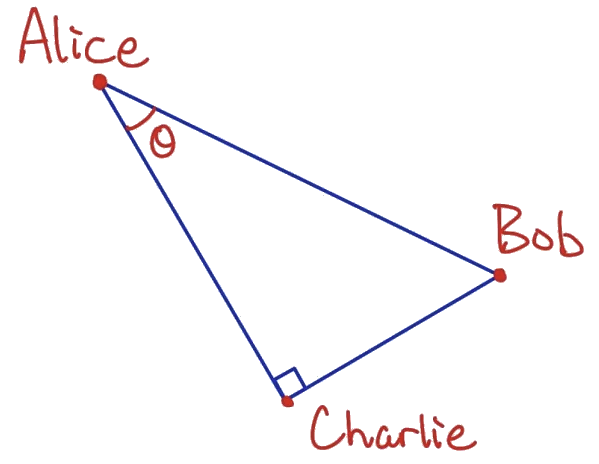
\includegraphics[scale=0.3]{triangle}
\end{center}

\textbf{Problem 3: (Make sure you include units in your final answers!)}  Using the figure shown, if the distance between Alice and Charlie is $4$ meters, and the distance between Charlie and Bob is $3$ meters, what is the distance between Alice and Bob? What is the angle $\theta$ in degrees? What is the angle $\theta$ in radian?\\
\newline\newline\newline
\newline\newline\newline
\newline\newline\newline
\newline\newline\newline
\newline\newline\newline

\textbf{Problem 4:} If $\theta = \pi/6$ in radian, and the distance between Alice and Bob is $10$ meters, what is the distance between Bob and Charlie?




\newpage
\textbf{Problem 1 (solution):}
I recommend first convert everything to the unit that you want, then do the algebra and computations, so we first we do 
\begin{align*}
r = 5 \text{ m} = \frac{5}{0.305}\text{ ft}\,,
\end{align*}
then we calculate the area
\begin{align*}
A = \pi r^2 = \pi \cdot \left( \frac{5}{0.305} \text{ ft}\right)^2= \pi \cdot \left( \frac{5}{0.305} \right)^2 \text{ ft}^2 \approx 844 \ \text{ft}^2\,.
\end{align*}
Make sure you have the correct unit in your final answer. For this class, when it comes to decimal places, I recommend keeping $3$ or $4$ significant digits unless specified otherwise.\\

\textbf{Problem 2 (solution):}
We want to find the unit of $B$, and the units of all other quantities are known, so we rearrange the $F = \rho v^2 B$ formula to isolate $B$, 
\begin{align*}
B = \frac{F}{\rho v^2}\,,
\end{align*}
then we just plug in the units and get
\begin{align*}
[B] = \frac{\text{kg m/s}^2}{(\text{kg/m}^3)\cdot (\text{m/s})^2} = \text{m}^2\,. 
\end{align*}
Now we see that $B$ has the unit of m$^2$, which is something like an ``Area". \\

\textbf{Problem 3 (solution):}
To find the distance between Alice ($A$) and Bob ($B$), we use the ``Pythagorean theorem" for triangles (with $a$ being opposite side, $b$ being adjacent side, and $c$ being hypotenuse), which states that 
\begin{align*}
a^2 + b^2 = c^2\,.
\end{align*}
So we see
\begin{align*}
AB = \sqrt{AC^2 + BC^2} =\sqrt{3^2 + 4^2} \,\text{m} =5\, \text{m}\,.
\end{align*}
Don't forget to include units in your final answer. To find the angle $\theta$, you can choose to use either $\sin(\theta) = a/c$, or $\cos(\theta) = b/c$, or $\tan(\theta) = a/b$. Here I do it using the tangent function, 
\begin{align*}
\theta = \arctan\left(\frac{3}{4}\right) = 0.664\, \text{rad} = 36.87^\circ\,.
\end{align*}
You might be allowed to use a calculator during the exams, so make sure you know how to switch between radian and degree modes in your calculator, or otherwise you will need to convert between the two manually.\\

\textbf{Problem 4 (solution):}
Now we know that $\theta = \pi/6$ and $AB = 10$ m. The side $AB$ is hypotenuse and we want to figure out the length of the opposite side, so we use the sine function, 
\begin{align*}
\sin(\pi/6) = \frac{BC}{10\, \text{m}}\,,
\end{align*}
so we find 
\begin{align*}
BC = 10\cdot \sin(\pi/6) \ \text{m} = 5 \ \text{m}\,.
\end{align*}
Again, make sure you include the unit :)

\end{document}


